    
\section{Exploratory Analysis}

    %data was preprocessed as described in methods
    
    
    % The outcome of the EDA will have a major impact on how you analyze the data:
    %  – Sample outliers and noise: Should some samples be discarded?
    % Can I perform a meaningful test for different expression between different groups?
    % What factors (wanted/unwanted, observed/unobserved) should be included in the model?
    
    % • EDA is the first part of the analysis where you start drawing biological conclusions specific to a
    % given experiment.
    % – Does the data look like I expected/designed?
    % – Do I have batch effects?
    % – Subgroups?
    % • In DE you formalize your observations in the EDA to extract statistically valid results.
    % • The resulting DE analysis will serve as the foundation of biological interpretation of the data.

    
    

    \subsection{Main effect subgroups}

    There are three main effects by which breast cancer samples can be stratified into groups: morphology, stage and PAM50 molecular profile. PCA is able separate samples into tumour/normal sample clusters fairly well (shown as an example in Methods, Figure \ref{fig:pcamethod}. However, it is more interesting to apply PCA to explore variation coming from separating samples in different cancer classification groups.  
    
    PCA was applied to 969 samples (857T, 112N), which were divided into subgroups by three systematic effect groups (i.e. PAM50, tumour morphology, cancer stage), which subgroup sizes shown in Tables \ref{table:morphstage} and \ref{table:pam50counts}. \\
    Figure \ref{fig:pcapam50} shows the PCA plot of first two principal components, coloured by PAM50 molecular subtype groups. PC1 accounts for 11\% of the total variation in the data, and is driven by the differences between normal and cancer samples. PC2 accounts for 8.6\% of the variation, and characterises the variation among breast cancer subtypes. Firstly, Basal-like samples form a separate cluster (orange), which emphasises its complete dissimilarity at molecular level. Luminal A and Luminal B form a partially overlapping cluster (yellow and red), which is expected from the known similarities of these subtypes. HER2-enriched cluster (blue) is understandably located between Luminal B and Basal-like as it is known to share expression profiles with these two. And lastly, seeing Normal-like subtype (pink) overlapping with normal samples (green) as well as with Luminal A cancer subtype fits nicely with the fact that Normal-like subtype shares morphology with the former and IHC and molecular profile with the latter.    
    
    % PAM50 PCA plot 
            \begin{figure}[!h]
            \centering
            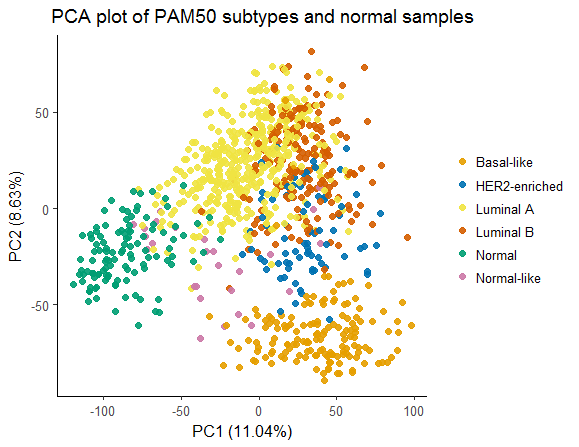
\includegraphics[scale=0.37]{pcapam502.png} 
            \caption{PCA plot showing the variance along PC1 and PC2 for PAM50 molecular subtypes of breast cancer and normal samples}
            \label{fig:pcapam50}
            \end{figure}
            
    \newpage
    Figure \ref{fig:1dpcapam50} shows the results of PCA for the first nine PCs, as described in the Methods section. Looking at the results in this way highlights again that PC1 is driven by tumour/normal variation. Together with PC2 they also capture the differences among PAM50 subtypes. As the PCs numbers increase, variation captured by them decreases. 
    
    % PAM50 1d PCA plot 
            \begin{figure}[!h]
            \centering
            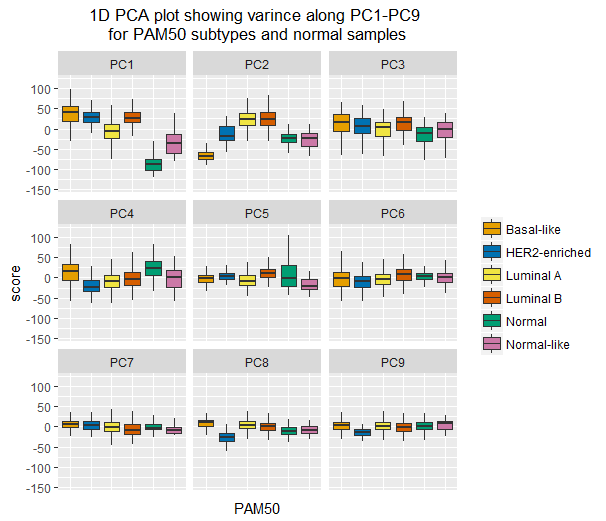
\includegraphics[scale=0.5]{1dpcapam50.png}
            \caption{One-dimensional PCA plots showing variance along PC1-PC9 for PAM50 molecular subtypes of breast cancer and normal samples. }
            \label{fig:1dpcapam50}
            \end{figure}
    
    
    The PCA results for morphology and stages classifications are shown in Figure \ref{fig:1dpcamorphstage} as one-dimensional variation plots. It can be observed that PCA was not able to capture as much variation between morphology groups and stages as among PAM50 subtypes. From one-dimensional plots it is evident that PC1 captures cancer/normal differences in both classification types. However, the rest of PCs do not capture enough variation to be evident on 2D PCA plots, therefore here only 1D plots are presented. Appendix \ref{} show 2D plots for results completion.    
    
    % 1D PCA for stages and morphology
            
            \begin{figure}[!h]
            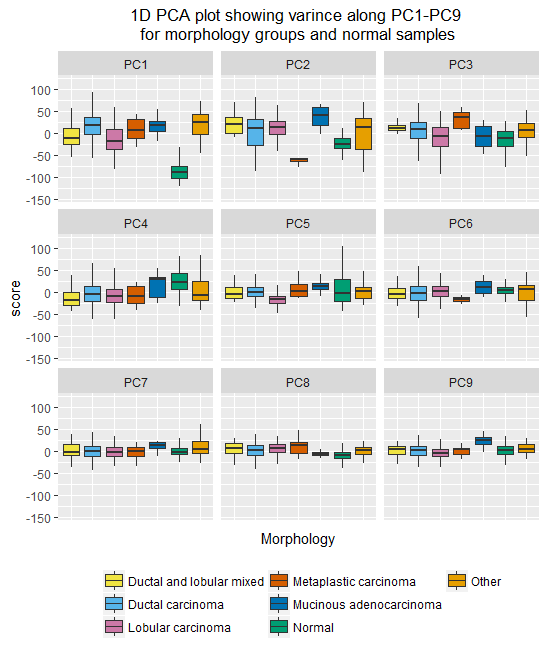
\includegraphics[width=0.4\linewidth]{1dpcamorph2.png}\hfill
            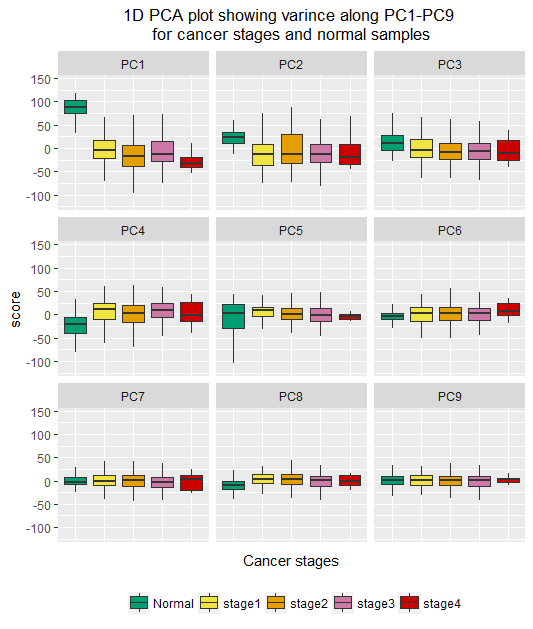
\includegraphics[width=0.4\linewidth]{1dpcastages2.png}
            \caption{One-dimensional PCA plots showing variance along PC1-PC9 for morphology groups and stages, with normal samples.}
            \label{fig:1dpcamorphstage}
            \end{figure}
            
    
    \newpage
    Interestingly, PCA was not able to capture any significant differences between stages (e.g. stage 1 and stage 4), where the differences in expression should be evident and therefore reflected in PCA results. The same is the case for two main distinct mythologies - Lobular and Ductal carcinomas, which overlap greatly. A possible explanation for these results is the unbalanced sizes of subgroups in these two classification methods, as well as their composition in terms of PAM50 subtypes, which is evidently the main driving force in sample classifications. 
    
    To explore this idea, the sample count data was visualised as stacked barplots presented in Figure \ref{fig:barms}. Each bar shows the total count of samples of a chosen morphology (left plot) or stage (right plot). The differing group sizes are evident.         
    
    % barsplots for stages and morphology 
       
        \begin{figure}[!h]
        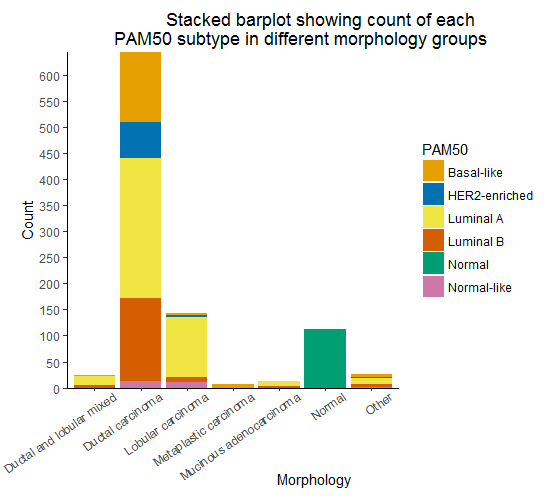
\includegraphics[width=0.53\linewidth]{bar_morph.png}\hfill
        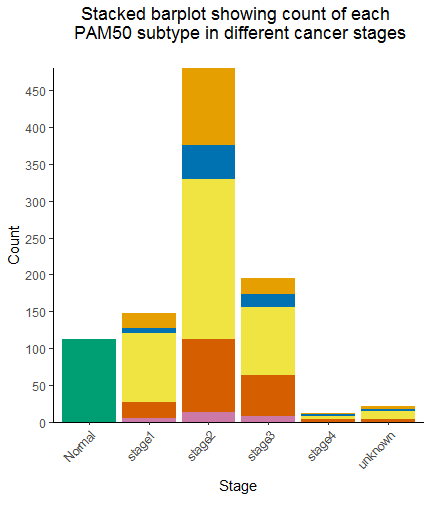
\includegraphics[width=0.4\linewidth]{bar_stages2.png}
        \caption{Stacked barplots of sample number counts per subgroups in morphology groups and stages classification groups. The coloured proportions represent PAM50 subtypes samples within each subgroup.}
        \label{fig:barms}
        \end{figure}
        
    Ductal carcinoma morphology samples make up over 70\% of all samples (x/857), but are well-proportionate in terms of PAM50 composition (i.e. similar proportions as the full dataset, with Luminal A dominating). Other subgroups, however, in addition to being smaller, are restricted to only a few PAM50 subtypes. For instance, Metaplastic carcinoma is made up completely of Basal-like samples, while Mucinous morphology is represented by only Luminal subtypes (the counts are shown in Table \ref{table:counts}). This observation explains why these two mophologies are separated in 1D PCA plot in PC2 (Figure \ref{fig:1dpcamorphstage}) - the difference between Luminal and Basal tissues is driving this variation. However, it is important to note, that there is a chance that these two morphologies, Metaplastic and Mucinous, actually only exists as Basal and Luminal subtype, respectively, but it is not possible to claim for or against this based on the current dataset.    
    
    The sample count difference between stages are also noticeable, which stage 2 accounting for roughly 50\% of the samples. The proportions of PAM50 subtypes within stages 1-3 appear to be well-balanced. Stage 4 is, however, of major concern. It has an alarmingly low sample count and is not represented in Normal-like subtype. The counts are shown in Table \ref{table:counts}.
        
        
    %TABLE x3 counts   
                \begin{table}[!h]
                \centering
                \caption{Samples number counts in pairwise comparisons of three main breast cancer samples classifications. Top table: PAM50 and stages, Middle table: PAM50 and morphology, Bottom table: stages and morphology. Each table shows row and column sums for each subgroup. The total count of samples in the project is in the lower right corner: 857.}
                \label{table:counts}      
                \resizebox{\textwidth}{!}{%
                \begin{tabular}{ccccccc}
                \multicolumn{1}{l|}{} & \multicolumn{1}{c|}{\textbf{Luminal A}} & \multicolumn{1}{c|}{\textbf{Luminal B}} & \multicolumn{1}{c|}{\textbf{Basal-like}} & \multicolumn{1}{c|}{\textbf{HER2-enriched}} & \multicolumn{1}{c|}{\textbf{Normal-like}} & {\color[HTML]{9B9B9B} \textit{rowsums}} \\ \hline
                \multicolumn{1}{c|}{\textbf{stage 1}} & \multicolumn{1}{c|}{94} & \multicolumn{1}{c|}{22} & \multicolumn{1}{c|}{21} & \multicolumn{1}{c|}{6} & \multicolumn{1}{c|}{5} & \multicolumn{1}{c|}{{\color[HTML]{656565} 148}} \\ \hline
                \multicolumn{1}{c|}{\textbf{stage 2}} & \multicolumn{1}{c|}{217} & \multicolumn{1}{c|}{99} & \multicolumn{1}{c|}{105} & \multicolumn{1}{c|}{47} & \multicolumn{1}{c|}{13} & \multicolumn{1}{c|}{{\color[HTML]{656565} 481}} \\ \hline
                \multicolumn{1}{c|}{\textbf{stage 3}} & \multicolumn{1}{c|}{93} & \multicolumn{1}{c|}{55} & \multicolumn{1}{c|}{21} & \multicolumn{1}{c|}{18} & \multicolumn{1}{c|}{8} & \multicolumn{1}{c|}{{\color[HTML]{656565} 195}} \\ \hline
                \multicolumn{1}{c|}{\textbf{stage 4}} & \multicolumn{1}{c|}{4} & \multicolumn{1}{c|}{4} & \multicolumn{1}{c|}{2} & \multicolumn{1}{c|}{2} & \multicolumn{1}{c|}{{\color[HTML]{C0C0C0} x}} & \multicolumn{1}{c|}{{\color[HTML]{656565} 12}} \\ \hline
                \multicolumn{1}{c|}{\textbf{unknown}} & \multicolumn{1}{c|}{12} & \multicolumn{1}{c|}{3} & \multicolumn{1}{c|}{4} & \multicolumn{1}{c|}{2} & \multicolumn{1}{c|}{{\color[HTML]{C0C0C0} x}} & \multicolumn{1}{c|}{{\color[HTML]{656565} 21}} \\ \hline
                \multicolumn{1}{c|}{{\color[HTML]{9B9B9B} \textit{colsums}}} & \multicolumn{1}{c|}{{\color[HTML]{656565} 420}} & \multicolumn{1}{c|}{{\color[HTML]{656565} 183}} & \multicolumn{1}{c|}{{\color[HTML]{656565} 153}} & \multicolumn{1}{c|}{{\color[HTML]{656565} 75}} & \multicolumn{1}{c|}{{\color[HTML]{656565} 26}} & \multicolumn{1}{c|}{\textit{857}} \\ \cline{2-7} 
                \multicolumn{1}{l}{} & \multicolumn{1}{l}{} & \multicolumn{1}{l}{} & \multicolumn{1}{l}{} & \multicolumn{1}{l}{} & \multicolumn{1}{l}{} & \multicolumn{1}{l}{} \\
                \multicolumn{1}{c|}{} & \multicolumn{1}{c|}{\textbf{Luminal A}} & \multicolumn{1}{c|}{\textbf{Luminal B}} & \multicolumn{1}{c|}{\textbf{Basal-like}} & \multicolumn{1}{c|}{\textbf{HER2-enriched}} & \multicolumn{1}{c|}{\textbf{Normal-like}} & {\color[HTML]{9B9B9B} \textit{rowsums}} \\ \hline
                \multicolumn{1}{c|}{\textbf{Lobular}} & \multicolumn{1}{c|}{114} & \multicolumn{1}{c|}{10} & \multicolumn{1}{c|}{3} & \multicolumn{1}{c|}{5} & \multicolumn{1}{c|}{11} & \multicolumn{1}{c|}{{\color[HTML]{656565} 143}} \\ \hline
                \multicolumn{1}{c|}{\textbf{Ductal}} & \multicolumn{1}{c|}{270} & \multicolumn{1}{c|}{158} & \multicolumn{1}{c|}{135} & \multicolumn{1}{c|}{68} & \multicolumn{1}{c|}{13} & \multicolumn{1}{c|}{{\color[HTML]{656565} 644}} \\ \hline
                \multicolumn{1}{c|}{{\color[HTML]{000000} \textbf{LobDuctal}}} & \multicolumn{1}{c|}{17} & \multicolumn{1}{c|}{6} & \multicolumn{1}{c|}{1} & \multicolumn{1}{c|}{{\color[HTML]{C0C0C0} x}} & \multicolumn{1}{c|}{{\color[HTML]{C0C0C0} x}} & \multicolumn{1}{c|}{{\color[HTML]{656565} 24}} \\ \hline
                \multicolumn{1}{c|}{\textbf{Metaplastic}} & \multicolumn{1}{c|}{{\color[HTML]{C0C0C0} x}} & \multicolumn{1}{c|}{{\color[HTML]{C0C0C0} x}} & \multicolumn{1}{c|}{7} & \multicolumn{1}{c|}{{\color[HTML]{C0C0C0} x}} & \multicolumn{1}{c|}{{\color[HTML]{C0C0C0} x}} & \multicolumn{1}{c|}{{\color[HTML]{656565} 7}} \\ \hline
                \multicolumn{1}{c|}{\textbf{Mucinous}} & \multicolumn{1}{c|}{8} & \multicolumn{1}{c|}{4} & \multicolumn{1}{c|}{{\color[HTML]{C0C0C0} x}} & \multicolumn{1}{c|}{{\color[HTML]{C0C0C0} x}} & \multicolumn{1}{c|}{{\color[HTML]{C0C0C0} x}} & \multicolumn{1}{c|}{{\color[HTML]{656565} 12}} \\ \hline
                \multicolumn{1}{c|}{\textbf{Other}} & \multicolumn{1}{c|}{11} & \multicolumn{1}{c|}{5} & \multicolumn{1}{c|}{7} & \multicolumn{1}{c|}{2} & \multicolumn{1}{c|}{2} & \multicolumn{1}{c|}{{\color[HTML]{656565} 27}} \\ \hline
                \multicolumn{1}{c|}{{\color[HTML]{9B9B9B} \textit{colsums}}} & \multicolumn{1}{c|}{{\color[HTML]{656565} 420}} & \multicolumn{1}{c|}{{\color[HTML]{656565} 183}} & \multicolumn{1}{c|}{{\color[HTML]{656565} 153}} & \multicolumn{1}{c|}{{\color[HTML]{656565} 75}} & \multicolumn{1}{c|}{{\color[HTML]{656565} 26}} & \multicolumn{1}{c|}{\textit{857}} \\ \cline{2-7} 
                \multicolumn{1}{l}{} & \multicolumn{1}{l}{} & \multicolumn{1}{l}{} & \multicolumn{1}{l}{} & \multicolumn{1}{l}{} & \multicolumn{1}{l}{} & \multicolumn{1}{l}{} \\
                \multicolumn{1}{c|}{} & \multicolumn{1}{c|}{\textbf{stage 1}} & \multicolumn{1}{c|}{\textbf{stage 2}} & \multicolumn{1}{c|}{\textbf{stage 3}} & \multicolumn{1}{c|}{\textbf{stage 4}} & \multicolumn{1}{c|}{\textbf{unknown}} & {\color[HTML]{9B9B9B} \textit{rowsums}} \\ \hline
                \multicolumn{1}{c|}{\textbf{Lobular}} & \multicolumn{1}{c|}{14} & \multicolumn{1}{c|}{78} & \multicolumn{1}{c|}{49} & \multicolumn{1}{c|}{{\color[HTML]{C0C0C0} x}} & \multicolumn{1}{c|}{2} & \multicolumn{1}{c|}{143} \\ \hline
                \multicolumn{1}{c|}{\textbf{Ductal}} & \multicolumn{1}{c|}{118} & \multicolumn{1}{c|}{368} & \multicolumn{1}{c|}{129} & \multicolumn{1}{c|}{11} & \multicolumn{1}{c|}{18} & \multicolumn{1}{c|}{644} \\ \hline
                \multicolumn{1}{c|}{\textbf{LobDuctal}} & \multicolumn{1}{c|}{5} & \multicolumn{1}{c|}{11} & \multicolumn{1}{c|}{7} & \multicolumn{1}{c|}{{\color[HTML]{C0C0C0} x}} & \multicolumn{1}{c|}{1} & \multicolumn{1}{c|}{24} \\ \hline
                \multicolumn{1}{c|}{\textbf{Metaplastic}} & \multicolumn{1}{c|}{2} & \multicolumn{1}{c|}{4} & \multicolumn{1}{c|}{1} & \multicolumn{1}{c|}{{\color[HTML]{C0C0C0} x}} & \multicolumn{1}{c|}{{\color[HTML]{C0C0C0} x}} & \multicolumn{1}{c|}{7} \\ \hline
                \multicolumn{1}{c|}{\textbf{Mucinous}} & \multicolumn{1}{c|}{3} & \multicolumn{1}{c|}{5} & \multicolumn{1}{c|}{4} & \multicolumn{1}{c|}{{\color[HTML]{C0C0C0} x}} & \multicolumn{1}{c|}{{\color[HTML]{C0C0C0} x}} & \multicolumn{1}{c|}{12} \\ \hline
                \multicolumn{1}{c|}{\textbf{Other}} & \multicolumn{1}{c|}{6} & \multicolumn{1}{c|}{15} & \multicolumn{1}{c|}{5} & \multicolumn{1}{c|}{1} & \multicolumn{1}{c|}{{\color[HTML]{C0C0C0} x}} & \multicolumn{1}{c|}{27} \\ \hline
                \multicolumn{1}{c|}{{\color[HTML]{9B9B9B} \textit{colsums}}} & \multicolumn{1}{c|}{148} & \multicolumn{1}{c|}{481} & \multicolumn{1}{c|}{195} & \multicolumn{1}{c|}{12} & \multicolumn{1}{c|}{21} & \multicolumn{1}{c|}{\textit{857}} \\ \cline{2-7} 
                \end{tabular}%
                }
                \end{table}

        
        
    \newpage  
    
    Another way of exploring the structure within a dataset and the relevance of different classification conventions is to perform sample clustering and visualise it as a heatmap. Figure \ref{fig:heatmap1k} shows the results of performing clustering on top 1000 highest variance genes. Variance was computed for each row (gene) in cancer samples only, and the top 1000 were selected to be used for clustering, as the genes with the most differences are of interest. The three main effect groups are shown above the heatmap as colour bars, which enables side-by-side comparisons.     
    
    % heatmap 1000
            \begin{figure}[!h]
            \centering
            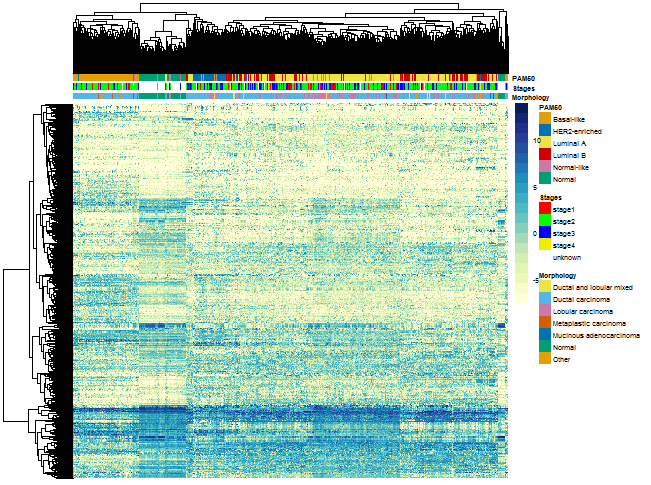
\includegraphics[scale=0.8]{heatmap_top1k.png}
            \caption{Heatmap with clustering on top 1000 highest variance genes (calculated on cancer samples only). The data is clustered by columns (samples) and rows (genes), with dendograms showing how clusters are formed. The colour bars above the heatmap (PAM50, stages, morphology) show the subgroups to which each sample belongs, colour-coded according to the legend on the right. The colours of heatmap represent gene expression intensity according to the scale (high expression - dark blue, low expression - light yellow). The data was clustered with Euclidean distance and average linkage. }
            \label{fig:heatmap1k}
            \end{figure}
    
    First and foremost, the unsupervised clustering was able to form two main clusters: Luminal and non-Luminal samples. Cluster on the right contains the majority of Luminal A and Luminal B samples according to the top colour bar (PAM50). The left hand side cluster contains Basal-like, HER2-enriched, and normal samples. Normal-like subtype is scattered across the entire dendogram, with more notable appearance inbetween Luminal A and normal samples, as expected. The Basal-like cluster is well-defined, which highlights this subtype difference from the rest. The Luminal types are mixed as anticipated. Overall, clustering is in line with the PCA results for PAM50 subtypes. \\
    With regards to stages and morphology colour bars, it can be observed that clustering, much like PCA, was not able to find any distinct major patterns among their subgroups. Again, the sizes of the subgroups may partially be responsible for that. It is a challenge to spot the minority-sized subgroups on the colour bar, and very clear to see how Ductal carcinoma dominates the dataset (light blue, third bar). The colour bar of stages also shows no distinct patterns. 
    
    \newpage
    However, another idea worth investigation is to test how data will cluster if sub-subgroups averages are taken. As stages of cancer progression are of high interest in this project, the averages of each PAM50 subtype at each stage were taken and clustered. Figure \ref{fig:dendogram} shows the resulting dendogram. 
    
        % dendogram
            \begin{figure}[!h]
            \centering
            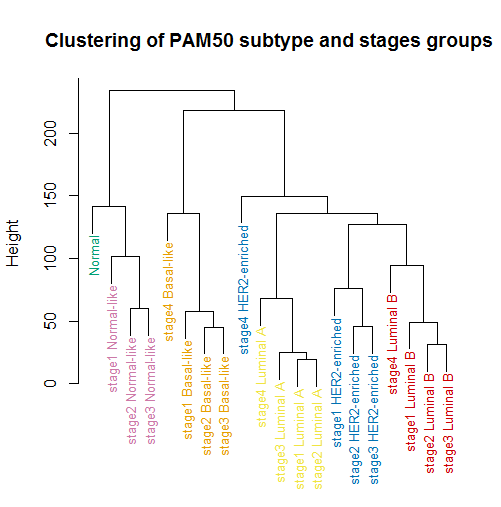
\includegraphics[scale=0.45]{dendogram2.png}
            \caption{Dendogram showing clustering of PAM50 subtypes within stages (averages per stage per subtypes)}
            \label{fig:dendogram}
            \end{figure}
    
    Remarkably, all subtypes form distinct branch clusters (expect HER2-enriched). Normal and Normal-like samples are the outgroup, understandably, and then Basal-like subtype is also an outgroup to the rest of samples. Luminal types and HER2-enriched are separated to well-defined branches. It is important to note that each subtype cluster has stage 4 branch as an outgroup, with the exception of HER2-enriched stage4, which is only made up of 2 samples perhaps leading to an unstable average. Seeing stage 4 as an outgroup is an important observation, as it is the most different and severe (due to metastasis) stage of cancer progression. \\
    
    Lastly, seeing the samples cluster primarily by PAM50 and only then by stage in Figure \ref{fig:dendogram}, is yet another evidence to what was observed with PCA and heatmap clustering. PAM50 is the main classification effect of breast cancer samples. When using other classification methods, PAM50 subtypes have to be taken into account. For example, comparing two morphologies might now produce expected results if their PAM50 subtype sample composition will be the main driving effect of differences. So the heterogeneity of groups has to be taken into account, and the downstream analysis has to be done on sub-subgroups.  
    
     

    
 
    
    \newpage
    \subsection{Cofactors and batch effects}
    
    Morphology, cancer stages, and PAM50 molecular subtype are the expected main sources of variation in the dataset, namely biological variation. However, in a large and heterogeneous dataset such as TCGA-BRCA there are potentially several other sources of variation that may be contributing to the differences in gene expression between samples. Having sufficient clinical and meta annotation for the present samples allows us to explore potential sources of technical variation.
    %AGE is a standard covariate
    Among the available annotations, the most interesting ones are the patient age group, year sample was taken, and tissue source site. These were explored with PCA to visualise any outlying subgroups that may be creating an unwanted batch effect.
    Exploring the samples by year may identify significant differences between years, as the lab protocols for sample processing would have changes in the given years (1988-2013). Such differences could also be observed between the source sites, i.e. clinical institutions and research centers where the original samples were handled. 

    One-dimensional PCA plots were used to visualise variation over the years and across the sample sites. As there are many (>20) subgroups in both year ans site data, PCA scatter plots are not helpful for spotting outlying subgroups. 
    
    Figure \ref{fig:1dpcayear} shows the first 6 PCs of PCA of the year data. Each boxplot represents samples taken in a single year, with individual years shown as gitter-dots to visualise each year group approximate size and sample variation within it (according to y-axis). The boxplots are shown for years in sequential order (1988-2013). 
        
            % 1D PCA YEAR
            \begin{figure}[!h]
            \centering
            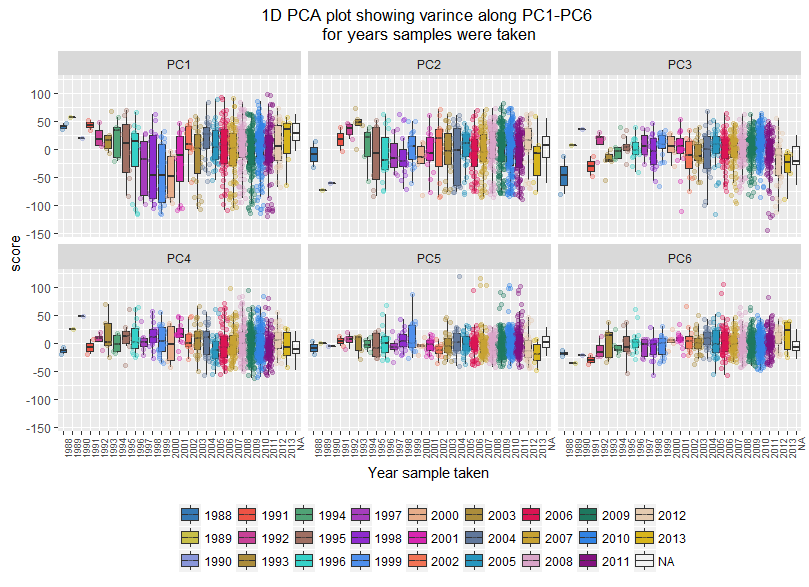
\includegraphics[scale=0.45]{1dpcayear.png}
            \caption{One-dimensional PCA plots showing variance along PC1-PC6 for all samples (cancer and normal) taken in years 1988-2013. The points over each box plot represent samples and their variation on the y-axis scale, to give a better indication of year group size and sample variation within it}
            \label{fig:1dpcayear}
            \end{figure}
    
    
    Overall, it is evident that there is a lot of variation between the years. This is especially the case for the earlier years, however, this is partially due to low number of samples taken in those years.  The variation stabilises after year 2005, which can be explained by the fact that this is when the pilot of TCGA project started and the universal protocols were introduced. Also it is can be seen that the majority of samples were collected after that time point. An observation worth noticing is that samples in years 1997-2000 appear to be quite different to previous and following years (PC1). This could have had a very serious batch effect on the downstream analyses, and had to be explored further.\\
    
    As established in the previous section, we expect PAM50 subtypes to be the main point of interest for further investigation, therefore, it was crucial to check the sample composition of every year group in terms of PAM50 subtypes to make sure that, for example, a particular subtype was *not*  collected in only one year, which would be confounding the dataset exploration in that context. Figure \ref{fig:baryear} shows the stacked barplot of all samples organised by year.  Each bar shows the total count of samples in a year, and the proportion of samples of each PAM50 subtype are coloured according to the legend. 
    
    
             % bar per year
            \begin{figure}[!h]
            \centering
            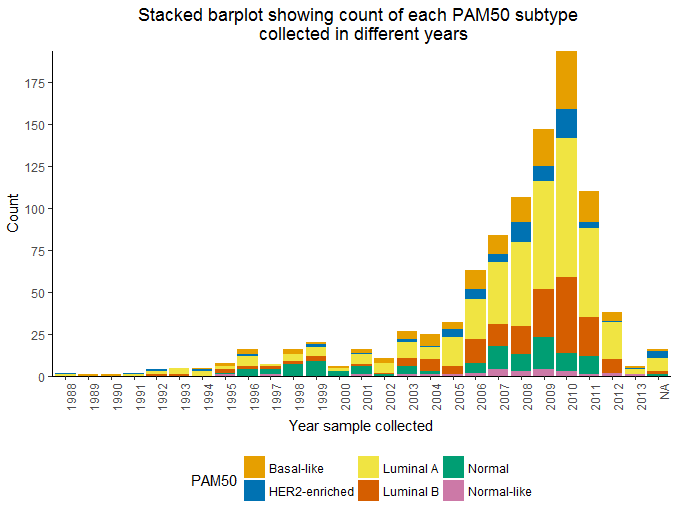
\includegraphics[scale=0.7]{bar_year.png}
            \caption{Stacked barplots of sample counts per year (1988-2013). The coloured proportions represent PAM50 subtypes samples within each year group. }
            \label{fig:baryear}
            \end{figure}
    
    As already noted from 1D PCA plot fro year data, the total number of samples in the earlier years is marginally smaller than in the last decade of given years. Overall, the distribution of PAM50 subtypes in each year is well-balanced,  although some years inevitably have no normal samples and/or samples of a specific subtype. On the whole, the dataset is not confounded by a particular year-subtype combination.  Moreover, visualising data in this way has shed light on the abnormality in years 1997-2000 seen in 1D PCA plot. It can be seen in Figure \ref{fig:baryear} that these years have about 50\% composition of normal samples in them, which is not the case for all other years. Having such high proportion of normal samples in them, makes their mean seem different. Appendix \ref{} shows a 1D PCA plot for cancer samples only, confirming this possible explanation, i.e. years 1997-2000 do not stand out from the rest if only cancer samples are included in the analysis. \\
    
        %sites
    \newpage
    As with year data, the sample source data also had to be explored and variation among sources assessed. Figure \ref{fig:1dpcatss} shows a 1D PCA plot analogous to the one showing variation for samples grouped by year. This plot shows variation for all samples grouped by samples source site (24 sites in total).\\  
            
            % 1D PCA YEAR
            \begin{figure}[!h]
            \centering
            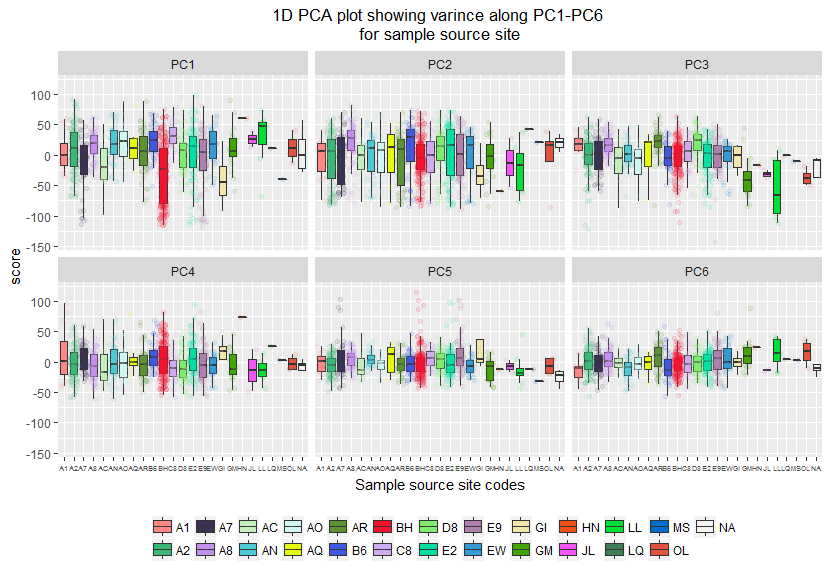
\includegraphics[scale=0.45]{1dpcatss.png}
            \caption{One-dimensional PCA plots showing variance along PC1-PC6 for all samples (cancer and normal) from different source sites (two letter abbreviations; NA - site unknown). The points over each box plot represent samples and their variation on the y-axis scale, to give a better indication of year group size and sample variation within it}
            \label{fig:1dpcatss}
            \end{figure}

    It is clear that the variation between source sites exists, as anticipated. As with year data, some source groups have very few samples, which makes the variation between them and large groups more prominent. One source site that really stands out (PC1) is BH (red). A possible explanation to this could have been that the sample handling protocol at this site is very different  from the rest, or, as it turned out, this differences has the same cause as the difference seen in year data.\\
    
              % bar per tss
            \begin{figure}[!h]
            \centering
            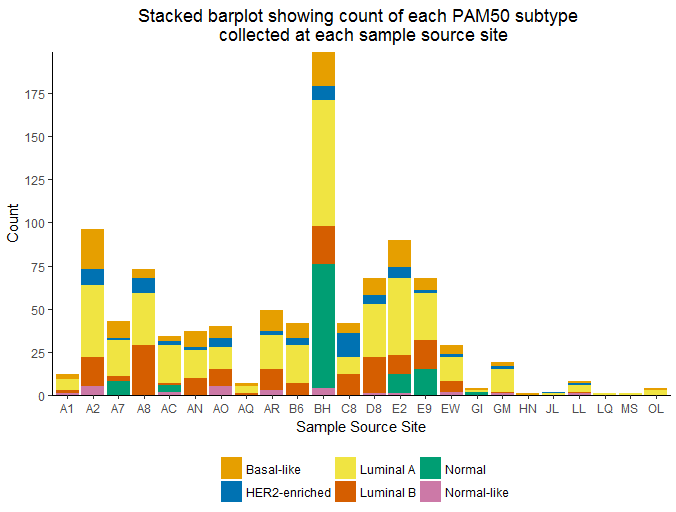
\includegraphics[scale=0.5]{bar_tss.png}
            \caption{Stacked barplots of sample counts per source site (alphabetic order). The coloured proportions represent PAM50 subtypes samples within each year group. }
            \label{fig:bartss}
            \end{figure}
    
    The source site data was visualised as stacked bar plots to inspect sample subtype variety coming from each site, Figure \ref{fig:bartss}. As observed on the 1D PCA plot, some sites have very few samples coming from them. The larger groups are relatively well-balanced in terms of their PAM50 subtype composition, with the exception of Normal-like, which comes only from 7 sites. This is, however, expected, as there are only 26 Normal-like samples in total. Another observation, which may be of bigger concern, is that the majority of normal samples come from one site, BH. This should not affect downstream analyses, as we are interested in differences between cancer subgroups. But seeing this explains the abnormal variation seen in 1D PCA plot for this site. As with year data, this one site is ~50\% composed of normal samples, making it appear very different from the rest as a group. If analysis is done only on cancer samples, this is no longer the case (Appendix \ref{}). 
    
  
    
    

    
    %age groups
    


\section{Looking for Autophagy signatures}

    \subsection{Differential Expression Testing}
    
        \subsubsection{Enrichment Analysis}

    \subsection{Soft clustering}
    
    %identify distinct transcriptome clusters
    %classify genes into groups
    
        \subsubsection{Enrichment Analysis}
    %     The expression profiles of these 348 genes were sorted into 5 clusters by using the fuzzy c-means algorithm implemented in the R package Mfuzz (20). The Mfuzz package uses a “fuzzy” clustering approach to compute the strength of the association of each gene with the central behavior of the cluster, referred to as a “fuzzy score.” The fuzzy scores for each gene sum to 1. This allows one to define a set of genes that associate with each cluster with a high probability, while other genes may not have a high score for association with a single cluster but may instead have scores that allow partial placement in more than one cluster. This approach is more flexible and less sensitive to experimental noise than traditional “hard” clustering, where each gene must belong to one and only one cluster.
 
% Table S1 in the supplemental material shows each of the 348 genes assigned to the 5 clusters and their individual fuzzy scores. The median fuzzy score for each cluster was >0.98, and the average fuzzy score was >0.9, indicating strongly correlated behaviors of the genes within each cluster with respect to changes in growth rate and substrate. Thus, each cluster has a core set of genes with very high fuzzy scores (i.e., close to 1) which indicate that their collective expression behavior is strongly correlated with that of other members of the cluster with respect to their changes in growth rate and substrate. Moreover, the lack of significant overlap of genes between the clusters also supports the unique characteristics of the clusters and their embedded genes.



 
% To overcome the limitations of hard clustering, soft clustering can be applied o
% ering several advantages to researchers [1, 2]. First, it generates accessible internal cluster structures, i.e. it indicates how well corresponding clusters represent genes/proteins. This additional information can be used for a rened search for regulatory elements. Second, the overall relation between clusters, and thus a global clustering structure, can be dened. Additionally, soft clustering is more noise robust and a priori pre-ltering of genes can be avoided. This prevents the exclusion of biologically relevant genes/proteins from the data analysis.



\section{Downstream}
